\chapter{Navigating Higher-dimensional Space}
\section{Graphically}
Navigating higher-dimensional space is of practical interest because a lot of
data is higher-dimensional, for example the field of machine learning for
example deals with very high dimensional data. Tools like `\verb|ggobi|' exist
to help explore multi-variate data \citep{swayne:dsc2003} which tend to
disregard spacial relations of points in favour of clustering based on shared
properties. %liu_2015

Whilst these approaches are useful for data, what we're dealing with here is
generating spaces to explore, these spaces are less about trends in data and
more about geometric exploration through many continuous parameters.

Video games also have explored non-euclidean and higher-dimensional spaces. An
interesting concept is that of 2D characters being able to navigate 3D spaces.
\emph{Super Paper Mario (2007)} for the Nintendo Wii is an example of this, the
player can turn the world 90 degrees about the y-axis to explore the depth of
the z-axis and progress through the game. An extension of this from a 3D
character turning 90 degrees and being able to explore a 4th Dimension is
present in the unreleased game \emph{Miegakure} in which the player can move
through the 4th Dimension using the controller, to help orient the player a
graphic \footnote{Which the developer tells me is based on an astrolabe} is
displayed below the controlled character showing the position of the slice of
the 4D world, these slices are like the 2D slices we can see in MRI imaging but
in 3D.

Whilst these worlds explore pre-made or procedurally generated assets, and this
program instead will explore moving through various parameters, ideas for how
the user can interface with the program to understand where exactly they are.

\subsection{Graphical Prompts}
A simple idea to allow the user to recall where in the parameter space they were
could be a spider / radar plot, or parallel coordinates plot. For our intents these
are the same as we're only displaying a single set of parameters the spider plot
is just a `round' version of the parallel coordinates plot. This could exist on
the screen somewhere and change as the user moved around the parameter space,
and would allow the user to recall approximately where they were. The spider
diagram could also be `extruded' from how it looked at every point to create a
3D model that represented how you moved through the parameters.

\subsection{Controls}
The above mentioned video games allow for the user to move through the space by
only letting the user worry about at most 3 dimensions at any one time, and
regarding the others as static when moving through them, this allows the user to
control the movement with traditional controls (either a games controller or
keyboard and mouse).

In \autoref{demomovement}, the \verb|WASD| style of control, popular in video
games is used. This will be familiar to people who have played video games but
not to people who haven't, for whom it may make sense to use the arrow keys.
It's also important to note that in that particular demo the `d' key increases
\verb|x|, this gives the feeling that the world is moving `beneath' you instead
of you moving the world itself; if the controls were flipped such that `d'
decreased \verb|x|, it would instead feel like you were moving the world. 

Another option would be something like an array of knobs, these could encode one
parameter each, and like a scientific instrument be `tuned'. However this relies
on specialist hardware. This would probably feel less like `moving' through a
space and more exploring a range of possibilities.

\section{Sonically}
\label{sonicnav}
I have developed a theoretical system for using sound to navigate a
higher-dimensional space, using ideas from \emph{Harry Partch} and \emph{Joe
Monzo's} approached to tuning theory.
\subsection{Intervals}
\begin{figure}[H]
    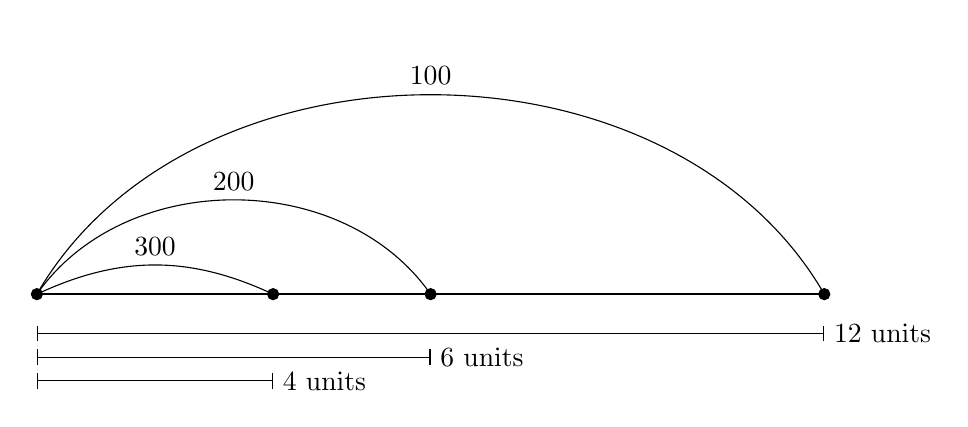
\begin{tikzpicture}
        %'string'
        \draw[-, thick] (-5, 0) -- (5, 0);
        \node at (-5, 0) {\pgfuseplotmark{*}};
        \node at (5, 0) {\pgfuseplotmark{*}};
        \node at (0, 0) {\pgfuseplotmark{*}};
        \node at (-2, 0) {\pgfuseplotmark{*}};
        
        % frequencies
        \draw[-, bend left=60] (-5, 0) to node[above] {$100\si{\hertz}$} (5, 0);
        \draw[-, bend left=55] (-5, 0) to node[above] {$200\si{\hertz}$} (0, 0);
        \draw[-, bend left=25] (-5, 0) to node[above] {$300\si{\hertz}$} (-2, 0);

        % lengths
        \draw[-, arrows=|-|] (-5, -0.5) -- (5, -0.5) node[right] {$12$ units};
        \draw[-, arrows=|-|] (-5, -0.8) -- (0, -0.8) node[right] {$6$ units};
        \draw[-, arrows=|-|] (-5, -1.1) -- (-2, -1.1) node[right] {$4$ units};
    \end{tikzpicture}
    \centering
    \caption{Diagram showing intervals being related to the idea of a ratio of
    lengths for example the $300\si{\hertz}$ frequency is related to the
    $200\si{\hertz}$ frequency by $\frac{6}{4} = \frac{3}{2}$}
\end{figure}

An \emph{interval} is simply a ratio of two frequencies: $\frac{f_1}{f_2}$.
This is a process to generate intervals based on a set of spacial coordinates,
or simply a set of parameters. Taking inspiration from the
\emph{just-intonation} tuning method a ratio comprised of integers only sounds
consonant. A \emph{$p$-limit} tuning system is a just-intonation based system
where every interval's highest prime factor is $p$. \citep[p.76,
109]{partch1974genesis}

3-limit tuning was the perhaps the first tuning system, being theorised by
Pythagoras and can be recreated by the ratios $\frac{3}{2}, \frac{2}{3},
\frac{1}{1}$. These can be represented using an exponent vector, usually called
a `monzo' \citep{monzo_2005}; for example $3:2$ is represented as such: $|-1\ 1\
\rangle$.  This is simply a shorthand for $2^{-1} 3^1$, and can be extended:
$|e_1\ e_2\ \cdots\ e_n\rangle$ where each $e_i$ in the vector is an exponent of
a prime number $2^{e_1} 3^{e_2} \cdots p_n^{e_n}$. 

Often these vectors are shown as $|*\ e_2\ \rangle$ The $*$ represents the idea
of octave equivalence, a musical idea that a doubling of the frequency produces
a note that is `the same', and as such any value of exponent for the $2$ can be
placed there. As an example $|1\ 1\rangle = 2^0 3^1 = \frac{3}{1}$ but this is
equivalent to $\frac{3}{2}$, as you can simply halve the frequency produced by
the ratio to get back to it. To normalise the interval the same octave, set the
constraints $1 \leq \frac{f_1}{f_2} < 2$ and similarly for other octaves higher
or lower, just halving and doubling the bounds.

\subsection{Navigating Space}
\subsubsection{In 2D}
Assume a base frequency, $440\si{\hertz} = f_1$. As an example, if the user was
at $x=1$, $y=-1$.

\begin{figure}[H]
    \centering
    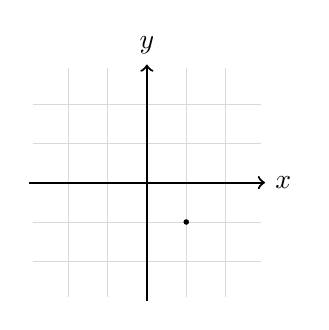
\begin{tikzpicture}[scale=0.5]
        \draw[help lines, color=gray!30](-2.9, -2.9) grid (2.9, 2.9);
        \draw[->, thick] (-3,0) -- (3,0) node[right]{$x$};
        \draw[->, thick] (0,-3)-- (0,3) node[above]{$y$};

        \fill (1,-1) circle[radius=2pt];
    \end{tikzpicture}
    \caption{}
\end{figure}

This is represented in the vector $|0\, 1\, -1\rangle$ which corresponds to $2^0
3^1 5^{-1} = \frac{6}{5}$. $\frac{6}{5}$ is a minor-third, and represents
$528\si{\hertz}$, this is consonant.

Or in general:
\begin{align*}
    2^n \cdot 3^x \cdot 5^y \cdot f_1 &= f_2
\end{align*}

If the user is at non-integer numbers for $x$ and $y$ we can calculate the frequencies too.
\begin{figure}[H]
    \centering
    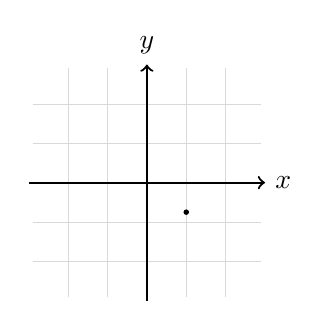
\begin{tikzpicture}[scale=0.5]
        \draw[help lines, color=gray!30](-2.9, -2.9) grid (2.9, 2.9);
        \draw[->, thick] (-3,0) -- (3,0) node[right]{$x$};
        \draw[->, thick] (0,-3)-- (0,3) node[above]{$y$};

        \fill (1,-0.75) circle[radius=2pt];
    \end{tikzpicture}
    \caption{}
    \label{outoftune}
\end{figure}

Where $x=1$ and $y=-0.75$ we can simply find the frequency as $2^0 \cdot 3^1
\cdot 5^{-0.75} \cdot 440\si{\hertz} = 394.772\si{\hertz}$. This will sound
dissonant and not particularly nice, perhaps the image produced by the program
will look disordered.

The idea here is simple, generating intervals like this allows for some points
in space to be consonant and others to be dissonant, these could correspond
visually with some output being produced by the program but should hopefully
allow a user to differentiate between points in space using their sense of
hearing.

\subsubsection{In Higher Dimensions}
This idea extends into higher dimensions naturally, simply adding to the number
of terms in the vector $|*\ e_3\ e_5\ \cdots\, e_p\  \rangle$. Each of these
exponents could represent some parameter added to the program. 

\subsection{Limitations}
As more variables are introduced integer ratios will sound less `strongly
consonant' and may be harder to understand naturally. However, every interval
that is possible with less variables will still be possible so a user could
still explore one or two parameters at a time and get the same results.

%TODO create appendix
\subsection{Processing Demo}
I have created a demo of this concept in 2D in processing, the code is in
\autoref{audiodemo}. The program simply has a integer-marked grid that the user
can navigate using \verb|WASD| and will calculate the interval based on the
coordinates of the point. Similarly to \autoref{outoftune}:

\begin{figure}[H]
\centering
\subfloat{\tikz[remember
picture]{\node(1AL){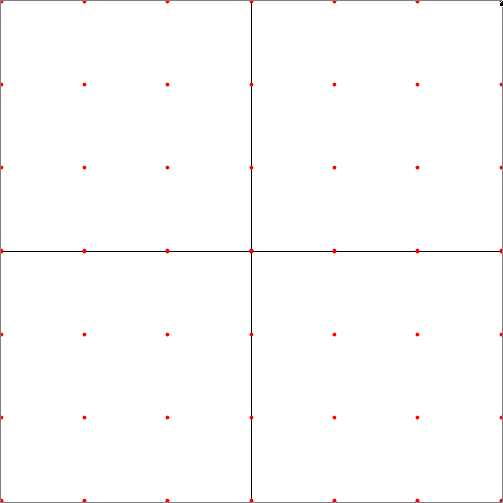
\includegraphics[width=.4\textwidth]{audiopoc2}};}}%
\hspace*{2cm}%
\subfloat{\tikz[remember
picture]{\node(1AR){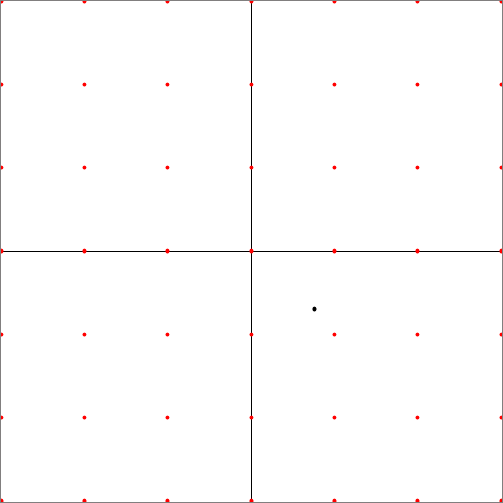
\includegraphics[width=.4\textwidth]{audiopoc1}};}}
\caption{At first the black dot is hidden beneath the centre red dot, the user uses WASD to navigate,
the audio is out of tune in the second state}
\end{figure}
\tikz[overlay,remember picture]{\draw[-latex,thick] (1AL) -- (1AL-|1AR.west)
node[midway,below]{};} 

This demo is very simple and only uses two sine waves so is very unpleasant to
listen to, but illustrates the point, at points outside those marked there is a
`beating' sound to the waves as they do not harmonise correctly. However, there
are points that aren't marked that \emph{do} sound somewhat consonant, so this
cannot be the only method for navigation, only a prompt to help the user.
